
%%%%%%%%%%%%%%%%%%%%%%%%%%%%%%%%%%%%%%%%%%%%%%%%%%%%%%%%%%%%%%%%%%%%%%%%%%%%%%%%

%        1         2         3         4         5         6         7         8

\documentclass[letterpaper, 10 pt, conference]{ieeeconf}  % Comment this line out if you need a4paper

%\documentclass[a4paper, 10pt, conference]{ieeeconf}      % Use this line for a4 paper

\IEEEoverridecommandlockouts                              % This command is only needed if 
                                                          % you want to use the \thanks command

\overrideIEEEmargins                                      % Needed to meet printer requirements.


\usepackage{graphics} % for pdf, bitmapped graphics files
\usepackage{epsfig} % for postscript graphics files
\usepackage{mathptmx} % assumes new font selection scheme installed
\usepackage{times} % assumes new font selection scheme installed
\usepackage{amsmath} % assumes amsmath package installed
\usepackage{amssymb}  % assumes amsmath package installed

\usepackage[font=small,labelfont=bf]{caption}

% Other package
\usepackage{tikz}
\usepackage{graphicx}
\usepackage{caption} 
\usepackage{subcaption}
\usepackage{multirow}
\usepackage{array}
\usepackage{booktabs}
\usepackage{hyperref}

\usepackage{pdfpages}
\usepackage{caption}
%\usepackage{geometry}
\usepackage{import}
\usepackage{standalone}

\title{\LARGE \bf
  Team-JSK: MBZIRC Progress Report
}
\author{Team JSK$^\dagger$% <-this % stops a space
  \\ JSK Lab, Graduate School of Information Science and Technology, The University of Tokyo \\
  7-3-1 Hongo, Bunkyo-ku, Tokyo, Japan 113-8656.  \\
\thanks{$^{*}$ %JSK Lab, Graduate School of Information Science and Technology, The University of Tokyo,  7-3-1 Hongo, Bunkyo-ku, Tokyo 113-8656, Japan.  
{$^\dagger$\tt\small http://www.jsk.t.u-tokyo.ac.jp}
}}
\begin{document}

\maketitle
\thispagestyle{empty}
\pagestyle{empty}


\section{INTRODUCTION}
This document provides a report of Team JSK's progress in preparing
for the Mohamed Bin Zayed International Robotics Challenge
(MBZIRC). The team consists of members from the JSK Laboratory at the
University of Tokyo. The JSK Lab, founded in early 1980’s, has a long
history of robotics research with focus on areas including humanoids,
drones, robotics manipulation, and perception, and the lab has
experience in participating in robotics challenges including the DARPA
Robotic Challenge and the Amazon Picking Challenge. JSK lab is also an
active contributor to the ROS community.


\section{PROJECT PERSONNEL}
Team JSK is made of eleven members: Prof. Masayuki Inaba, Prof. Kei
Okada, Dr. Yohei Kakiuchi, Dr. Wesley Chan, Bakui Chou, Xiangyu Chen,
Krishneel Chaudhary, Kohei Kimura, Yuki Furuta, and Hiroto
Mizohana. The team is roughly divided into three groups corresponding
to each task with groups having overlapping personnel.


%That is a professor, a associate-professor, a lecturer, a researcher, 4 Phd students and 2 Master students. 
%Teachers mainly focus on manage the whole team schedule, design hardware and software architecture, provide advices and give ideas for all the tasks. The rest researcher and students are divided into three groups, 
%one for computer vision development for all the tasks, one for task 2 and one for task 1 and 3.


\section{CHALLENGE 1: LANDING UAV ON A MOVING VEHICLE}


%Copyright (C) 2016 by Krishneel@JSK Lab, The University of Tokyo

%Copyright (C) 2016 by Krishneel@JSK Lab, The University of Tokyo

\documentclass{standalone}
\usepackage{footnote}
\usepackage{hyperref}
\usepackage{graphicx}
\usepackage{fancyhdr}

\renewcommand\footnoterule{%
  \kern-3\p@
  \hrule\@width2.5cm
  \kern2.6\p@
}
\makeatother

\begin{document}

\section{Software}


\subsection{Software Environment}
The motion planning and visual perception algorithms are implemented
on Robot Operating System (ROS) environment\footnote{\url{http://www.ros.org}}.
We used Gazebo\footnote{\url{gazebosim.org}} for virtual simulations
\footnote{\url{https://github.com/start-jsk/jsk_mbzirc}}. Our
algorithms are implemented in C/C++, Python and CUDA-C.


\subsection{Visual Perception}

The image processing is one of the fundamental component of autonomous
systems. With efficient and robust image processing the planning and
decision making can be done more readily which improves the accuracy
and robustness of executing the assigned task. Hence, one of our
primary objective while designing our software architectures was
real-time performance with minimal loss of accuracy. The visual
components of task one include three main stages described as follows:

\subsubsection{Target Detection}
The target detection phase is the initial localization of the landing
region (heliport) on the truck. To detect the heliport we use the
traditional computer vision detection approach where by a sliding
window based method is used. However such raster scanning windows are
computationally expensive even for high end systems. To overcome this
crucial limitation we first generate candidate objectness
regions. Since the heliport is fixed to a moving target, we use
Gaussian based background subtractor fused with Kalman Filters for 
global motion compensation to generate regions of interest
(ROI)  with stable changes. The candidate ROI's are then ranked using
edge similarity between each sliding window. High scoring ROI are then
used for detecting the heliport using pretrained detector. 
Let $\mathbf{H}$ denote the detected target region.

\subsubsection{Target Tracking}

In order for an UAV to approach and land on the heliport online visual
feedback is very important given that the target is constantly moving.
Using the assumption that the target is not
expected to change abruptly both in terms of visual motion and
appearances, we use visual tracking for online feedback.
The detected region $\mathbf{H}$ is used to initialize the
tracker. Our visual tracking algorithm is highly efficient and robust
to both scale and visual changes and runs in real time, thus
providing frame by frame location of the target. To enable a tracker
to run online in real time we carefully crafted the expensive process
of feature computation by reducing it to one time process. 
The invariant features for tracking are computed by passing the image
through several pre-trained kernels of varying dimensions. By varying
the sizes of the kernel, an approximate scale can also be detected.
Moreover, the tracker is updated online at fixed intervals.

\begin{figure}[t!]
  \centering
  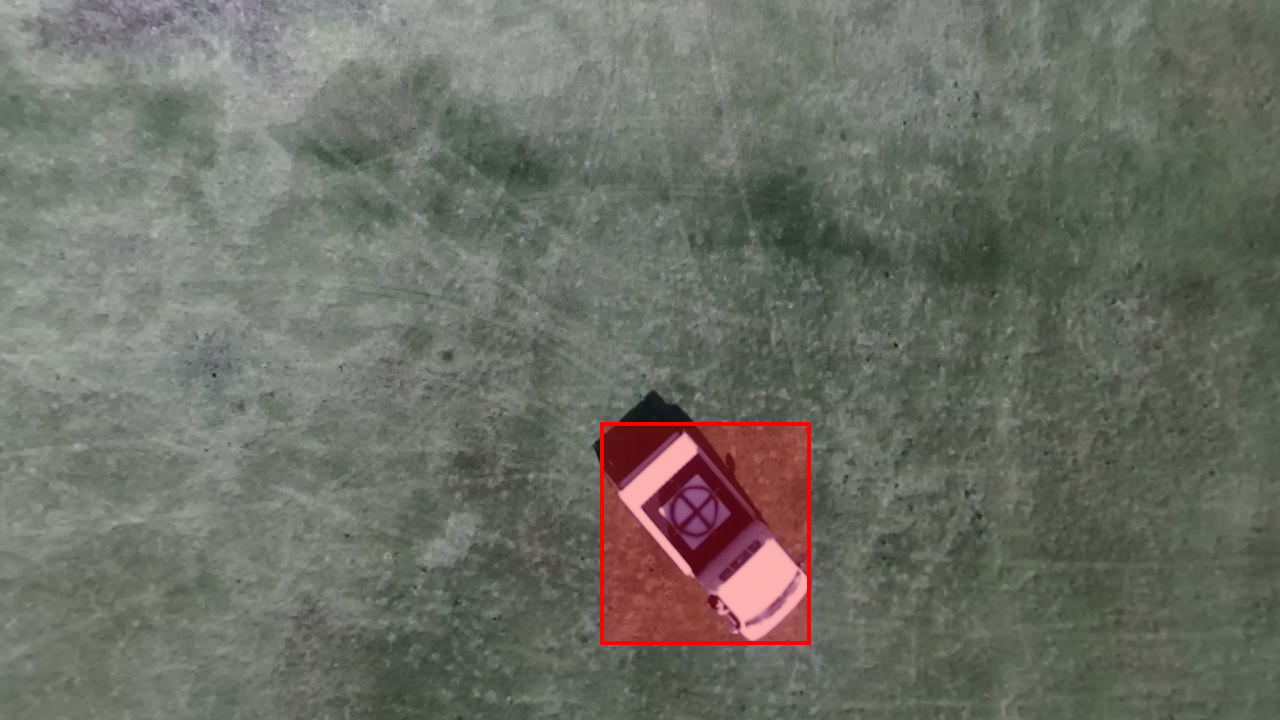
\includegraphics[height=1in]{sections/task1/images/detect2}
  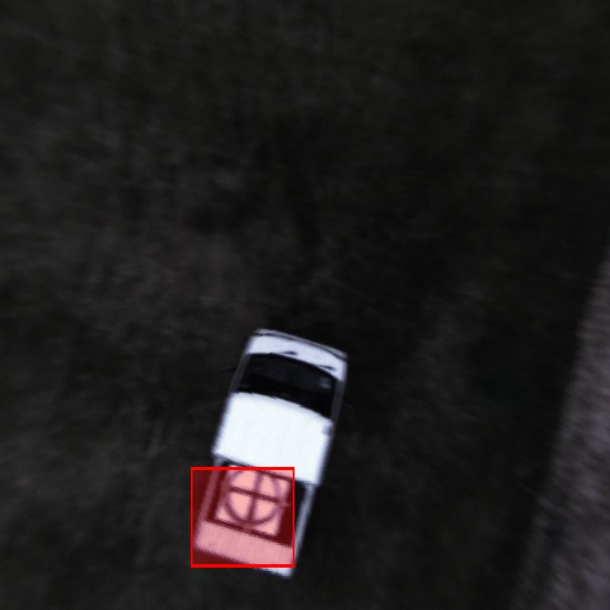
\includegraphics[height=1in]{sections/task1/images/detect1}
  \caption{Illustration of truck and heliport detection.}
\end{figure}

\subsection{Control Method}

\subsubsection{Landing Control}
Our landing algorithm is closely cooperating with our robust tracking algorithm. We defined an inverted conical region related to the center of object. When UAV is stably moving in this region, UAV is considered tightly keeping in tracking with the moving object. Then UAV starts going down with stable speed. And our strategy is that when UAV is 0.3 meter higher than truck, we will stop going down and adjust to the most center of the parking apron and land directly and quickly to it. The reason is that currently our tracker in vision algorithm is to detect the inside circle region of parking apron, whose radius is 0.5 meter, and the look-down fisheye camera we used is 120 degree for perspective, so it means when UAV is 0.29 meter higher than parking apron, look-down camera could not cover the whole region. But 0.29 meter is already close enough for UAV to directly land, and our experiments also prove this strategy is practically feasible.


\subsection{Results Achieved to Date}

We have completed task one fully autonomously landing on the moving
target at 5km/h, 10km/h and 15km/h. The results of these landings are
shown in video. Moreover we demonstrate the effectiveness of our real
time planning and tracking by showing the results of long time
following of the target at over 35km/h.

For landing control, we first test our method to land on fixed truck, and result shows that precision is below 10 centimeters, which is close to an start-of-the-work by HKUST's team in ICRA2015. And for moving object, we succeeded ladning on truck with 15, 10 and 5 Km/h as shown in our attached video.

\subsection{Future Work}
\subsubsection{Landing Control}
Since outdoor landing when target object is moving in high speed is an unsolved difficult problem, currently our landing is also restricted in straight-road landing. However in the challenge, starting from center crosswords, only a 20-meter straight road is available. If considering truck is moving with 15 Km/h (~4 m/s), UAV has to land within 5 seconds. Currently for development and safety consideration, our landing is slow and need around 15 seconds.
In next stage, we plan to reevaluate this academic problems and make pioneer trails to generate realtime landing trajectory for landing during target object is turning with high speed.


\end{document}


%% insert yout latex module file here. the contents should go to the tasks folder under section

\section{CHALLENGE 2: OPERATING A VALVE STEM}

%Copyright (C) 2016 by Krishneel@JSK Lab, The University of Tokyo

\documentclass{standalone}
\begin{document}

\section{example}

This example.tex shows how to write the module


\end{document}

\section{CHALLENGE 3: SEARCH, PICK AND PLACE}

%Copyright (C) 2016 by Krishneel@JSK Lab, The University of Tokyo

\documentclass{standalone}
\begin{document}

\subsection{Platforms}

\end{document}


\section{GRAND CHALLENGE}

%Copyright (C) 2016 by Krishneel@JSK Lab, The University of Tokyo

\documentclass{standalone}

\usepackage{graphicx}
\usepackage{float}
\floatstyle{boxed} 
\restylefloat{figure}

\begin{document}


\begin{figure*}[!b]
   \newcommand \ilenght{0.1}
   \newcommand \iheight{2.0in}
   \newcommand \iwidth{0.23\textwidth}
   \centering
   
   \subcaptionbox{
     \scriptsize{}\label{fig3:a}}{\includegraphics[width=\iwidth, height=\iheight]{sections/grand/images/DJI_0028}}\hspace{1.1em}%
   \subcaptionbox{
     \scriptsize{}\label{fig3:b}}{\includegraphics[width=\iwidth, height=\iheight]{sections/grand/images/DJI_0059}}\hspace{1.1em}%
   \subcaptionbox{
     \scriptsize{}\label{fig3:c}}{\includegraphics[width=\iwidth, height=\iheight]{sections/grand/images/DJI_0079}}\hspace{1.1em}%
   \subcaptionbox{
     \scriptsize{}\label{fig3:d}}{\includegraphics[width=\iwidth, height=\iheight]{sections/grand/images/DJI_0092}}\hspace{1.1em}%
   \caption{JSK--Team testbed setup at Hachioji, Tokyo, Japan}
   \label{fig:objects}
 \end{figure*}


\subsection{Setup of TestBed}

We have prepared our testbed where we will perform the outdoor testing in the real world is located in Hachioji, Tokyo, Japan. 

 \subsection{Future Work}
 Once we complete each of the three tasks above, for the grand challenge we will combine each of the 3 tasks above, however we plan to make some changes such as UAV to UAV and UAV to UGV communications such that all the robots are able to collaborate in completing the tasks.
 

\end{document}

%\section{Future Plan}

\end{document}
